\documentclass[10pt,a4paper]{standalone}
\usepackage[utf8]{inputenc}
\usepackage[T1]{fontenc}
\usepackage{amsmath}
\usepackage{amsfonts}
\usepackage{amssymb}
\usepackage{graphicx}

\usepackage{tikz}
\usepackage{pgfplots}
\pgfplotsset{compat=1.13}

\pgfplotsset{
	width=150mm,height=100mm,
	major grid style={thin,dotted,color=black!50},
	minor grid style={thin,dotted,color=black!50},
	grid,
	every axis/.append style={
		line width=0.5pt,
		tick style={
			line cap=round,
			thin,
			major tick length=4pt,
			minor tick length=2pt,
		},
	},
	legend cell align=left,
	legend pos=north west,
}

\begin{document}
%	\title{Radix sort}
%	\date{}
%	\maketitle
	
	% IMPORT-DATA rsort compare_sort.txt
	
	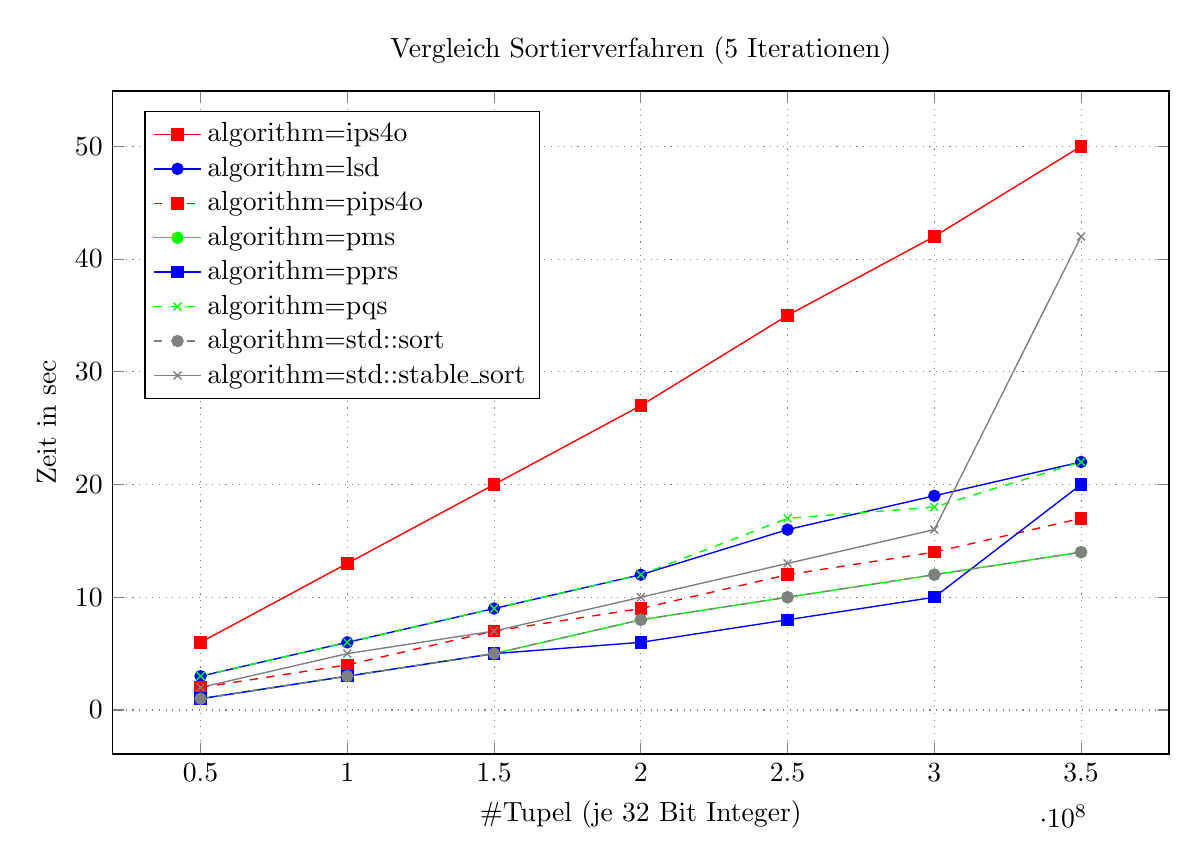
\begin{tikzpicture}
		\begin{axis}[
		title={Vergleich Sortierverfahren (5 Iterationen)},
		xlabel={\#Tupel (je 32 Bit Integer)},
		ylabel={Zeit in sec},
		]
		
		%% MULTIPLOT(algorithm) SELECT elements AS x, (SUM(time) / 5000) AS y, MULTIPLOT
		%% FROM rsort GROUP BY MULTIPLOT,x ORDER BY MULTIPLOT,x
  \addplot[red, mark=square*, mark options={solid}] coordinates { (50000000,6) (1e+08,13) (1.5e+08,20) (2e+08,27) (2.5e+08,35) (3e+08,42) (3.5e+08,50) };
  \addlegendentry{algorithm=ips4o};
  \addplot[blue, mark=*, mark options={solid}] coordinates { (50000000,3) (1e+08,6) (1.5e+08,9) (2e+08,12) (2.5e+08,16) (3e+08,19) (3.5e+08,22) };
  \addlegendentry{algorithm=lsd};
  \addplot[dashed, red, mark=square*, mark options={solid}] coordinates { (50000000,2) (1e+08,4) (1.5e+08,7) (2e+08,9) (2.5e+08,12) (3e+08,14) (3.5e+08,17) };
  \addlegendentry{algorithm=pips4o};
  \addplot[green, mark=*, mark options={solid}] coordinates { (50000000,1) (1e+08,3) (1.5e+08,5) (2e+08,8) (2.5e+08,10) (3e+08,12) (3.5e+08,14) };
  \addlegendentry{algorithm=pms};
  \addplot[blue, mark=square*, mark options={solid}] coordinates { (50000000,1) (1e+08,3) (1.5e+08,5) (2e+08,6) (2.5e+08,8) (3e+08,10) (3.5e+08,20) };
  \addlegendentry{algorithm=pprs};
  \addplot[dashed, green, mark=x, mark options={solid}] coordinates { (50000000,3) (1e+08,6) (1.5e+08,9) (2e+08,12) (2.5e+08,17) (3e+08,18) (3.5e+08,22) };
  \addlegendentry{algorithm=pqs};
  \addplot[dashed, gray, mark=*, mark options={solid}] coordinates { (50000000,1) (1e+08,3) (1.5e+08,5) (2e+08,8) (2.5e+08,10) (3e+08,12) (3.5e+08,14) };
  \addlegendentry{algorithm=std::sort};
  \addplot[gray, mark=x, mark options={solid}] coordinates { (50000000,2) (1e+08,5) (1.5e+08,7) (2e+08,10) (2.5e+08,13) (3e+08,16) (3.5e+08,42) };
  \addlegendentry{algorithm=std::stable\_sort};
		
		\end{axis}
	\end{tikzpicture}
\end{document}
